\documentclass[12pt]{article}
\usepackage[margin=1in]{geometry}
\usepackage{graphicx}
\usepackage[export]{adjustbox}
\usepackage{mathtools}
\renewcommand{\baselinestretch}{1.5}
\title{BCI - Cybathalon Race Report}
\date{\today}
\author{Sjoerd Bos, Stef Brands, Jelmer Jansen, Theo Pijkeren}
\begin{document}
\pagenumbering{gobble}
\maketitle
\newpage
\pagenumbering{arabic}
\section{Introduction}
\subsection{What is a BCI?}
A Brain Computer Interface (BCI) is a system which allows someone to communicate information about their mental state without the use of the peripheral nervous system. The main purpose of this is to aid people how have lost control of some of their motor functions and are thus unable to perform certain actions. This can be communication, but also walking or moving their arms. A prime example of the use of BCI for communication is the visual speller. With this users can choose letters from a roster whilst only using their brains. Another example of a good working BCI is a system that allows a man that has lost control of his arm, to move it again by thinking about certain movements.
 \begin{figure}[h]
 	\caption{p-300 visual speller and arm control BCI}
 	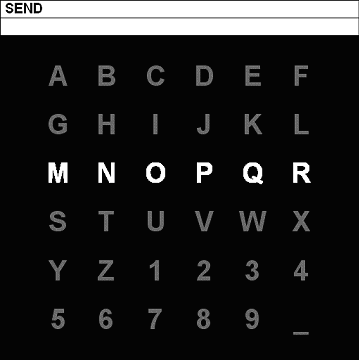
\includegraphics[scale=0.5]{VisualSpeller.png}
 	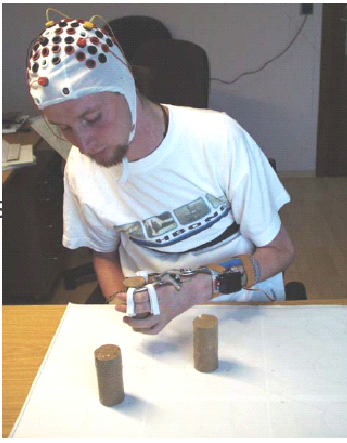
\includegraphics[scale=0.5]{InducedBCI.png}
 \end{figure}

\subsection{Cybathalon}
The cybathalon is an event in which people with physical disabilities can 'race' against each other in various disciplines with the aid of technology. One of these is the brainrunners event. 'Brainrunners' is a computer game in which the users can control their character purely with their brain. This game is played with 4 different commands for 4 different parts of the course. Each command should be a distinct signal from the brain. For this game one should use 3 or 4 induced responses and potentially 1 rest. If the user produces the response corresponding to the color that his avatar is currently on than it will go fast. If no command is send the character will move at normal speed, but if a wrong command is send the character will go very slow. In the end, the user with the fastest time wins.
	\begin{figure}[h]
		\caption{The brainrunners game}
		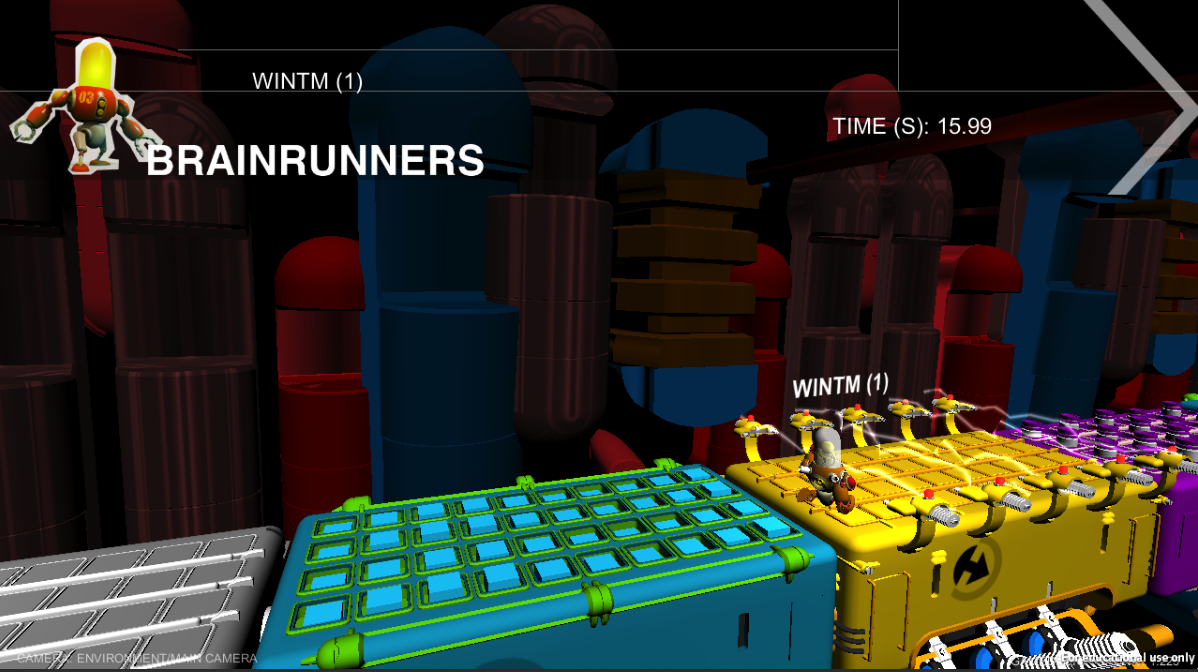
\includegraphics[scale=0.3]{Brainrunners.png}
	\end{figure}

\subsection{Aim of the research}
The aim of this research is to experiment with different setups for brainrunners and figure out which one is the most successful. This report will be specifically focused towards task selection, electrode placement, subject selection and state of the subject at the time of playing the game. We will use a Mobita EEG system with 10 electrodes for this experiment. 

\section{Method}
\subsection{Subject Selection}
We searched for multiple subjects to use for the BCI Cybathalon Race. We did a training session on multiple people from our own group. The classifier returns the classification accuracy and we did the following training sessions on the subject that has the highest accuracy. The subject we selected from our group was Theo Pijkeren. 

\subsection{Task Selection}
We first tried training our subject on imagined movement. There were three explicit classes and one rest class. The classes were $feet$, $left hand$, $right hand$ and $rest$. The subject thinks about the corresponding movements. The moments between the imagined movements were used for the $rest$ class. We noticed that our subject had a relatively good classification accuracy on all classes except for the $rest$ class. Therefore we decided to replace the $rest$ class with a fourth imagined movement, namely tongue movement. We trained our subject multiple times with these four classes. However, the three classes with a rest class eventually resulted in a higher accuracy. 

\subsection{Electrode Placement}
The ten electrodes were first placed more or less all around the scalp. We noticed that only the electrodes that were placed at the center of the head, were contributing to a good classification. 

\begin{figure}[h]
 	\caption{EEG graphs with electrodes placed all around the scalp}
 	\label{fig:eeg1}
 	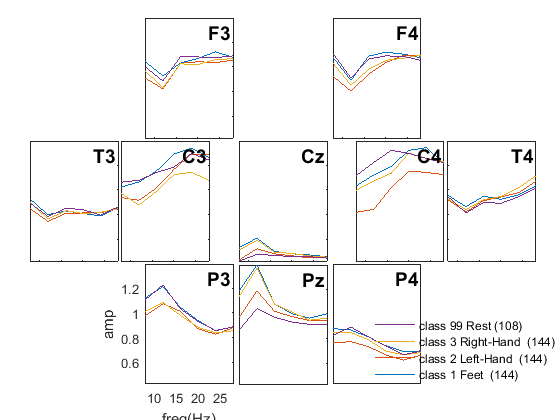
\includegraphics[scale=0.6,center]{eeg_graphs.png}
\end{figure}
 
 You see in Figure \ref{fig:eeg1} that there is only a clear distinction between the classes in the electrodes in the center of the head ($C5, C4$ and $Pz$). We decided to place the electrodes that did not contribute that much to the classifier at different locations, more centered around the middle of the head. We moved electrodes $F3, F4, T3$, and $T4$.
 
 \begin{figure}[h!]
 	\caption{EEG graphs with electrodes placed mostly around the center of the scalp}
 	\label{fig:eeg2}
 	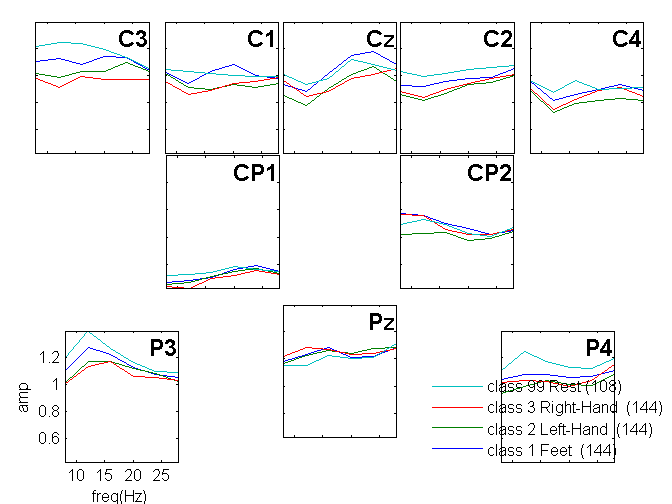
\includegraphics[scale=0.6,center]{eeg_graphs2.png}
 \end{figure}
 
 We kept the electrodes $P3, Pz$ and $P4$ at the same place, because they cover the visual areas of the brain. Our subject imagined himself moving his hands and feet visually in combination with imagining the physical, kinetic movement. The former is covered by the electrodes at the back of the head. The later covers the imagined kinetic movements. The new electrode placement is shown in Figure \ref{fig:eeg2}.

\subsection{Meditation}


\end{document}